\subsection{Testing}

\begin{multicols}{2}


With the proposed implementation of the framework, we get the following search results given the "city map data set" test data. Which can be seen on the right. 

As the map is to scale with the given locations, street names are quite small, but when viewed on a device, it should be possible to zoom in and view details if interested.

For testing, it will be interesting to see if directional uni-directional streets are respected, as well as if the map finds the shortest path if possible.

First, we can try to check if the algorithm can find the trivial path from a crossing to the same crossing. As an example, the initial and goal crossing is set to be the crossing between "Vestervoldgade" and "Vestergade". The expected output from here should be an empty list of street names, as no street is needed to be travelled to reach the destination. This matches the actual output, as seen in figure \ref{fig:test1}.

\begin{figure}[H]
    \centering
    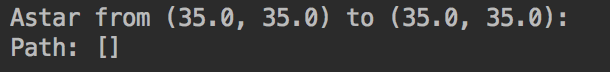
\includegraphics[width = 0.9\linewidth]{RouteFinding/RFtest1.png}
    \caption{Trivial route from crossing to same crossing result.}
    \label{fig:test1}
\end{figure}


\begin{figure}[H]
  \begin{center}
    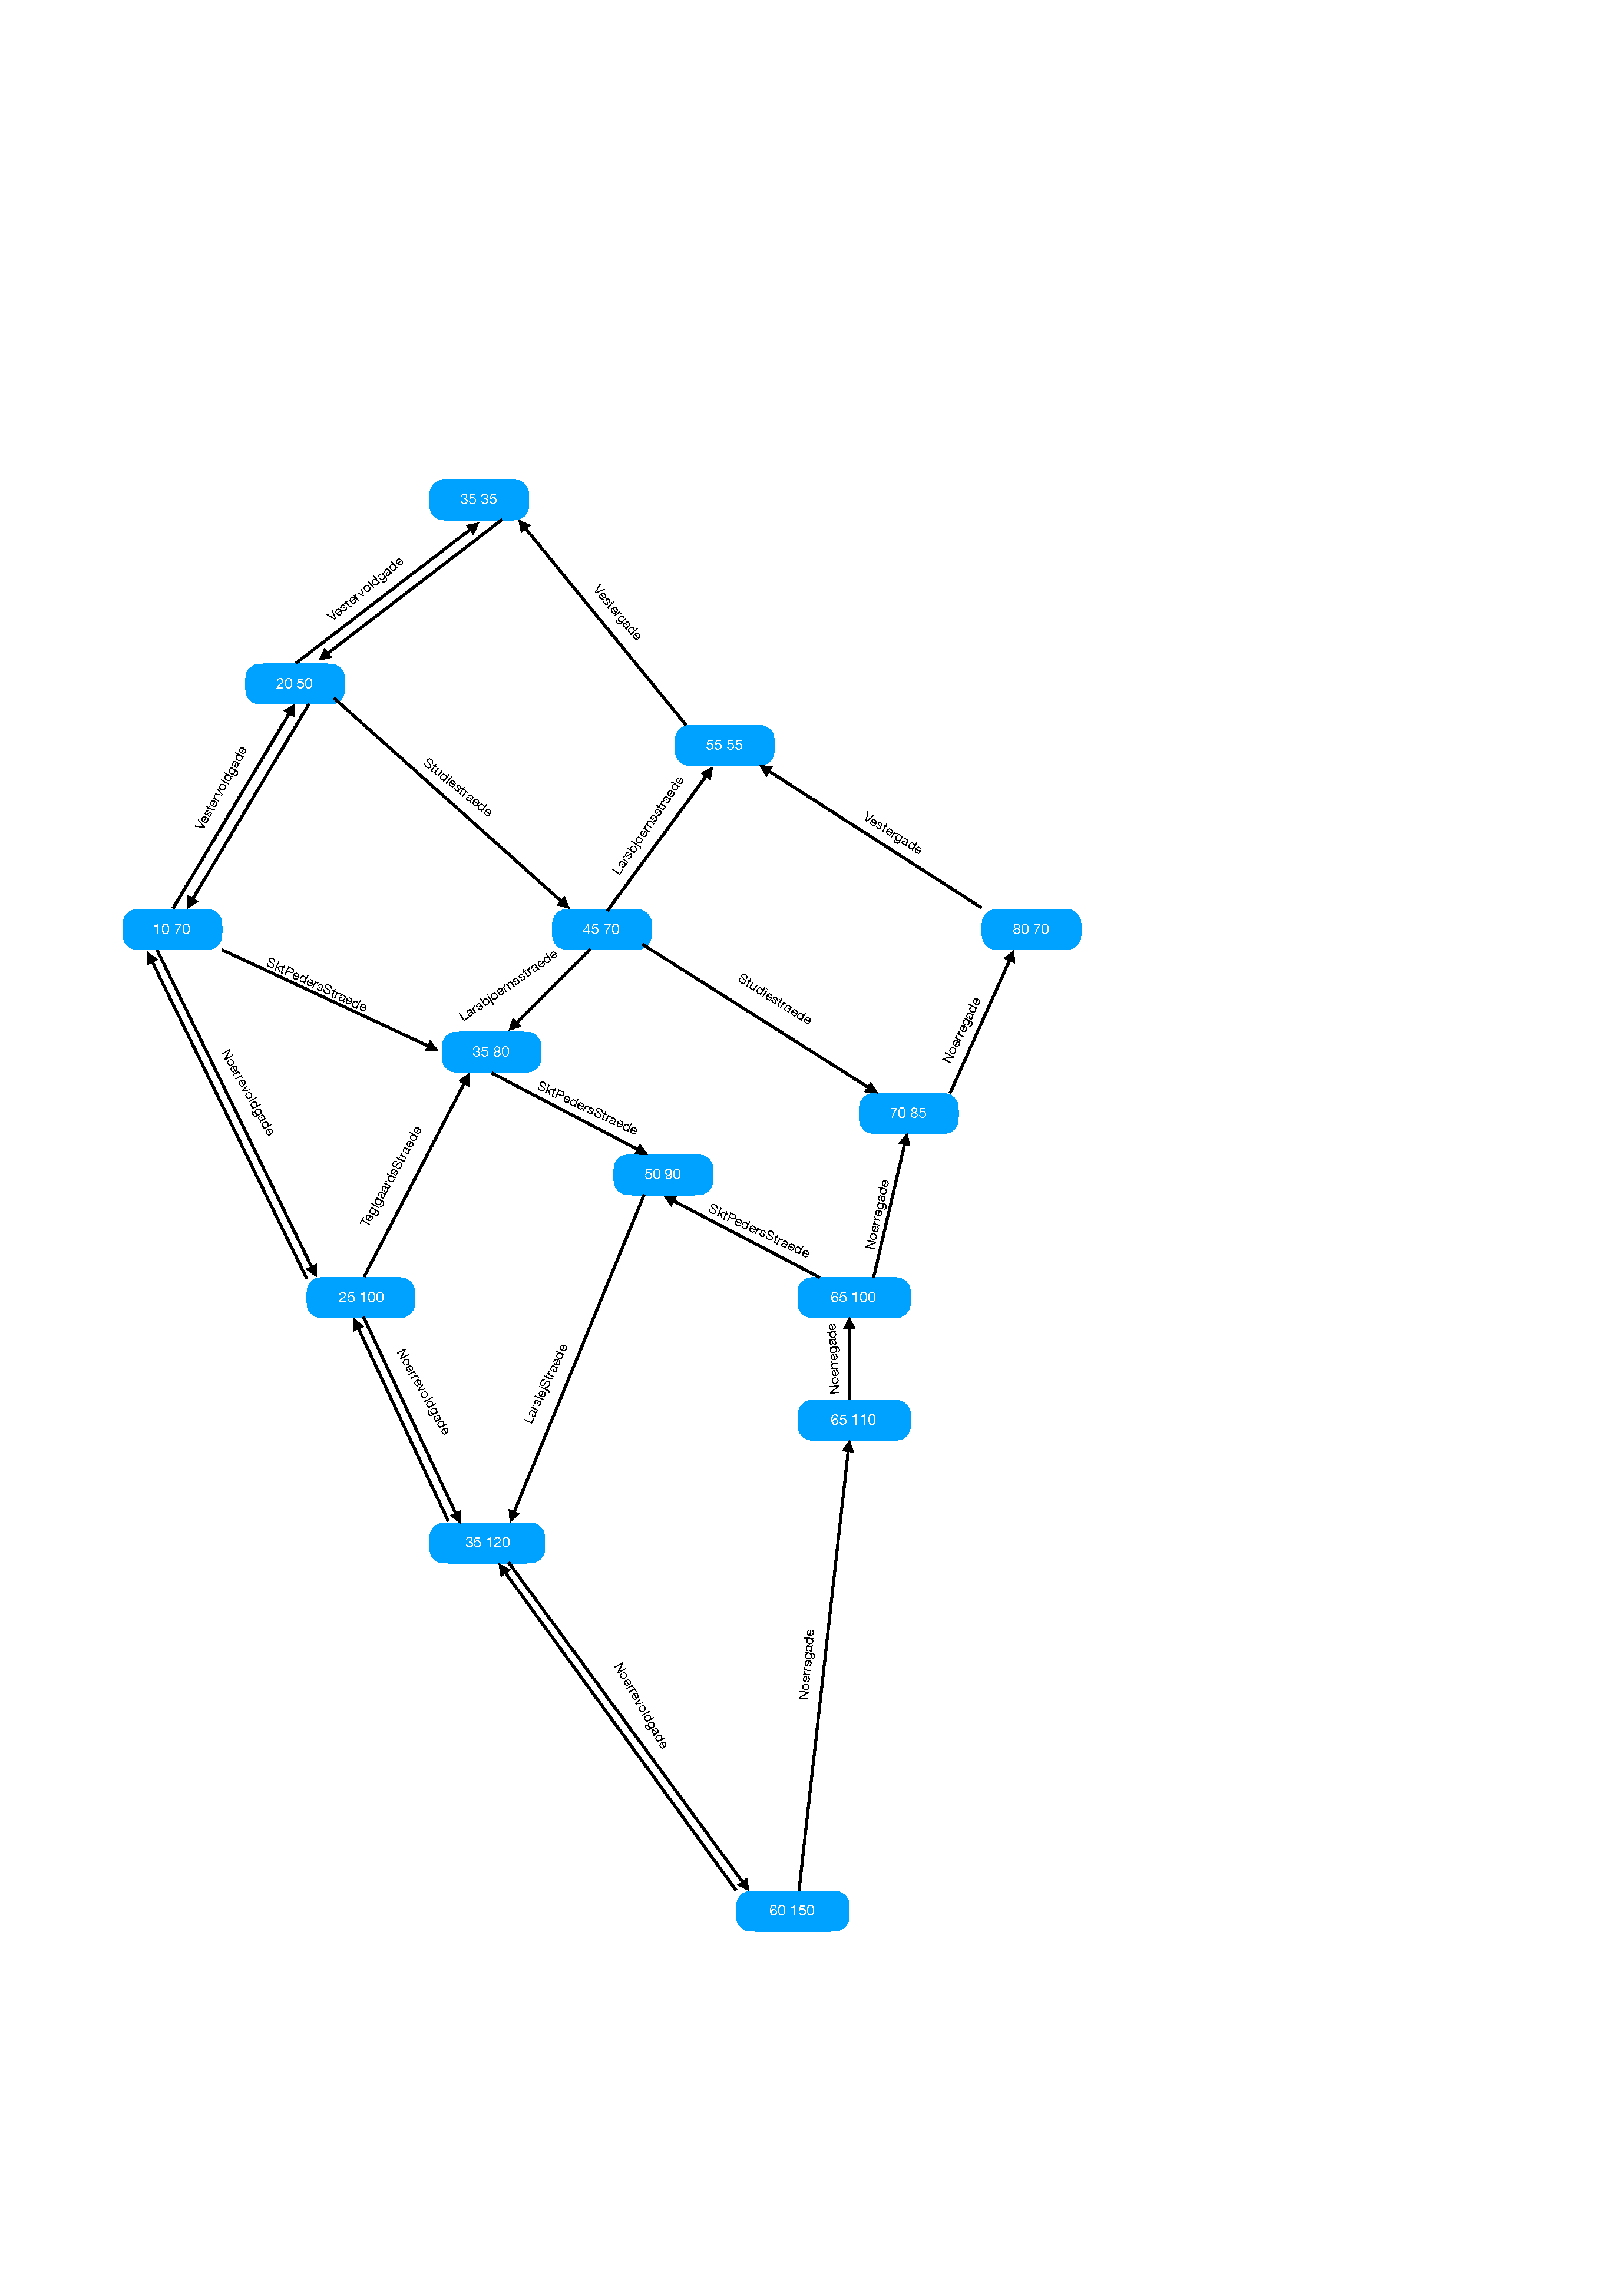
\includegraphics[width=0.9\linewidth]{RouteFinding/CityMap.pdf}
  \end{center}
  \caption{City Map}
\end{figure}

\end{multicols}

Next we test if the algorithm respects uni-directional streets. The example here is from the crossing between "Noerregade" and "Studiestraede", to the crossing between "Studiestraede" and "Larsbjoernsstraede". The expected output is, the path all the way around following the streets "Noerregade", "Vestergade", "Vestervoldgade" and "Studiestraede". This matches the actual output as seen in figure \ref{fig:test2}. Note that "Vestergade" is listed twice, as two travels along that street is performed.

\begin{figure}[H]
    \centering
    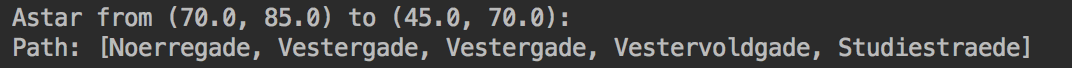
\includegraphics[width = 0.8\linewidth]{RouteFinding/RFtest2.png}
    \caption{Uni-directional street test result.}
    \label{fig:test2}
\end{figure}

Finally we want to test a route which has multiple possible paths, and verify that the output corresponds with the shortest possible path. The example here is from the crossing between "Vestervoldgade" and "Studiestraede", to the crossing between "SktPedersStraede" and "Noerregade".

Possible paths are and lengths are: \\
 $[$ "Vestervoldgade", "Noerrevoldgade", "Noerrevoldgade", "Noerrevoldgade", "Noerregade", "Noerregade" $]$
with a length of 157.62

$[$"Studiestraede", "Larsbjoernsstraede", "SktPedersStraede", "LarslejStraede", "Noerrevoldgade", "Noerregade", "Noerregade"$]$ 
with a length of 187.00

$[$"Vestervoldgade", "SktPedersStraede", "SktPedersStraede", "LarslejStraede", "Noerrevoldgade", "Noerregade", "Noerregade"$]$
with a length of 190.22

We expect to see the first path as output. This matches the actual output as seen in figure \ref{fig:test3}.

\begin{figure}[H]
    \centering
    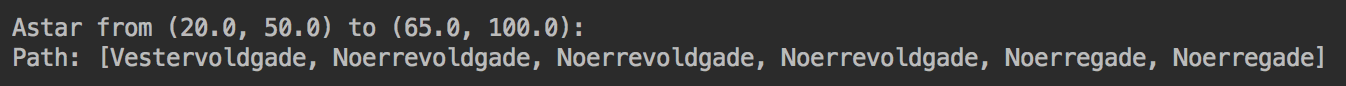
\includegraphics[width = 0.9\linewidth]{RouteFinding/RFtest3.png}
    \caption{Shortest path test result.}
    \label{fig:test3}
\end{figure}

Based on these tests, it is probable that the implementation of the A* algorithm is correct, as it has satisfied our behavioral expectations.